---
id: tkz-euclide-ejemplo-06
title: Punto Relativo
description: "Crea un punto a una distancia y dirección dadas respecto a otro (coordenadas polares)."
keywords: [puntos, desplazamiento, coordenadas-polares, direccion, distancia]
tags: [tkzDefPoint,tkzDefShiftPoint,tkzLabelPoints]
sort: 6
---
\documentclass[tikz,border=2mm]{standalone}
\usepackage{tkz-euclide}

\begin{document}
    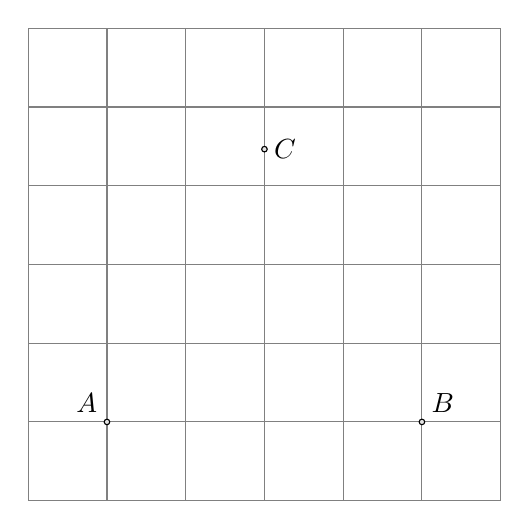
\begin{tikzpicture}
        % Define el sistema de coordenadas ortogonales.
        \tkzInit[xmin=0,xmax=6,ymin=0,ymax=6]
        % Dibuja los ejes del plano cartesiano.
        \tkzDrawXY
        % Dibuja una cuadrícula en el área definida.
        \tkzGrid
    
        % Define los puntos A y B.
        \tkzDefPoint(1,1){A}
        \tkzDefPoint(5,1){B}
    
        % Define el punto C a 4cm de A, a 60 grados.
        \tkzDefShiftPoint[A](60:4){C}
    
        % Dibuja los puntos A,B,C
        \tkzDrawPoints(A,B,C)
    
        % Etiqueta el punto A arriba a la izquierda.
        \tkzLabelPoints[above left](A)
        % Etiqueta el punto B arriba a la derecha.
        \tkzLabelPoints[above right](B)
        % Etiqueta el punto C a la derecha.
        \tkzLabelPoints[right](C)
    \end{tikzpicture}
\end{document}